%%%%%%%%%%%%%%%%%%%%%%%%%%%%%%%%%%%%%%%%%
% University/School Laboratory Report
% LaTeX Template
% Version 3.1 (25/3/14)
%
% This template has been downloaded from:
% http://www.LaTeXTemplates.com
%
% Original author:
% Linux and Unix Users Group at Virginia Tech Wiki 
% (https://vtluug.org/wiki/Example_LaTeX_chem_lab_report)
%
% License:
% CC BY-NC-SA 3.0 (http://creativecommons.org/licenses/by-nc-sa/3.0/)
%
%%%%%%%%%%%%%%%%%%%%%%%%%%%%%%%%%%%%%%%%%

%----------------------------------------------------------------------------------------
%	PACKAGES AND DOCUMENT CONFIGURATIONS
%----------------------------------------------------------------------------------------

\documentclass{article}

\usepackage{array}
\usepackage{tabularx}
\usepackage{geometry}
\usepackage{graphicx} % Required for the inclusion of images
\usepackage[utf8]{inputenc}
\usepackage[english]{babel}
\usepackage{minted}
\usemintedstyle{borland}
\usepackage{xcolor}
\setlength\parindent{1.2pt} % Removes all indentation from paragraphs

\renewcommand{\labelenumi}{\alph{enumi}.} % Make numbering in the enumerate environment by letter rather than number (e.g. subsection 6)
\geometry{
 a4paper,
 total={170mm,257mm},
 left=20mm,
 top=20mm,
 }
%\usepackage{times} % Uncomment to use the Times New Roman font

%----------------------------------------------------------------------------------------
%	DOCUMENT INFORMATION
%----------------------------------------------------------------------------------------

\title{
	Microcontroller Lab Report \\
\large 8086 programming Part 1
} % Title

\author{
	Aaditya Prakash Kattekola \\
	{\small Roll: 194201} \\
	{\small ECE Section B} \\
} % Author name

\date{August 28, 2021} % Date for the report

\begin{document}

\maketitle % Insert the title, author and date

% If you wish to include an abstract, uncomment the lines below
% \begin{abstract}
% Abstract text
% \end{abstract}

%----------------------------------------------------------------------------------------
%	Question 1
%----------------------------------------------------------------------------------------

\break
\section{Question 1}
%----------------------------------------------------------------------------------------
%	subsection 1
%----------------------------------------------------------------------------------------

\subsection{Aim}
Write the assembly language program for 8086 MP to add two 16-bit numbers.

%----------------------------------------------------------------------------------------
%	subsection 2
%----------------------------------------------------------------------------------------

\subsection{Program}
\subsubsection{Code}
\inputminted{nasm}{"C:/Users/aadit/Documents/BTech/5th Semester/MC Lab/8086 Pgrm 1/ADD.asm"}

\subsubsection{Emulator}

\begin{center}
\begin{tabularx}{1.0\textwidth} { 
  | >{\centering\arraybackslash}X 
  | >{\centering\arraybackslash}X 
  | >{\centering\arraybackslash}X | }
 \hline
\textbf{Address  (CS:0100, IP:0000)} &\textbf{Machine code}&\textbf{Instruction} \\
  \hline
 01000 & B8,01,00 & MOV AX, 00001H \\ 
  \hline
   01003 & BB,00,25 & MOV BX, 02500H \\ 
  \hline
   01006 & 03, C3 & ADD AX, BX \\  
  \hline
  01008 & F4 & HLT \\  
  \hline
\end{tabularx}
\end{center}

%----------------------------------------------------------------------------------------
%	subsection 3
%----------------------------------------------------------------------------------------
\break
\subsection{Result}
\subsubsection{Input}
AX: 0001H \\
BX: 2500H \\

\subsubsection{Expectation}
AX $\leftarrow$ AX+BX; \\  
0001H+2500H $\rightarrow$ 2501H in AX \\

%----------------------------------------------------------------------------------------
%	subsection 4
%----------------------------------------------------------------------------------------

\subsubsection{Emulator}

\begin{figure}[h]
\begin{center}
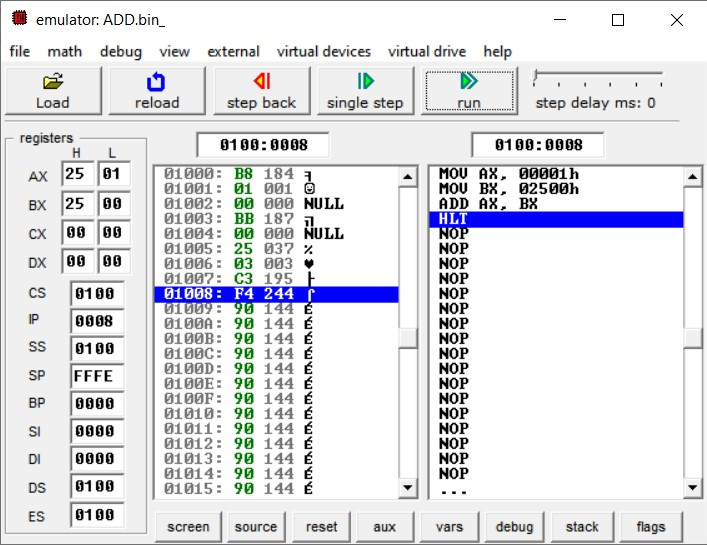
\includegraphics[width=1.0\textwidth]{ADD} 
\caption{STACK Output for Q1}
\end{center}
\end{figure}




%----------------------------------------------------------------------------------------
%	Question 2
%----------------------------------------------------------------------------------------

\break
\section{Question 2}
%----------------------------------------------------------------------------------------
%	subsection 2
%----------------------------------------------------------------------------------------

\subsection{Aim}
Write the assembly language program for 8086 MP to count even and odd numbers in an array of numbers stored in memory.

%----------------------------------------------------------------------------------------
%	subsection 2
%----------------------------------------------------------------------------------------

\subsection{Program}
\subsubsection{Code}
\inputminted{nasm}{"C:/Users/aadit/Documents/BTech/5th Semester/MC Lab/8086 Pgrm 1/EVEN_ODD_COUNT.asm"}

\subsubsection{Emulator}

\begin{center}
\begin{tabularx}{1.0\textwidth} { 
  | >{\centering\arraybackslash}X 
  | >{\centering\arraybackslash}X 
  | >{\centering\arraybackslash}X | }
 \hline
\textbf{Address  (CS:0100, IP:0000)} &\textbf{Machine code}&\textbf{Instruction} \\
  \hline
 01000 & BE, 00, C9 & MOV SI, 0C900H \\ 
  \hline
   01003 & B1, 04 & MOV CL, 04h \\ 
  \hline
   01006 & BB, 00, 00 & MOV BX, 00000H \\  
   \hline
   01005 & BB, 00, 00 & MOV BX, 00000H \\
   \hline
   01008 & 8A, 04 & MOV AL, [SI] \\
   \hline
   0100A & F8 & CLC \\
   \hline
   0100B & D0, C8 & ROR AL, 1 \\
   \hline
   0100D & 72, 04 & JB 013H \\
   \hline
   0100F & FE, C7 & INC BH \\
    \hline
   01011 & EB, 02 & JMP 015H \\
    \hline
   01013 & FE, C3 & INC BL \\
    \hline
   01015 & 46 & INC SI \\
   \hline
   01016 & FE, C9 & DEC CL \\
   \hline
   01018 & 75, EE & JNE 0108H \\
  \hline
  01008 & F4 & HLT \\  
  \hline
\end{tabularx}
\end{center}

%----------------------------------------------------------------------------------------
%	subsection 3
%----------------------------------------------------------------------------------------
\break
\subsection{Result}
\subsubsection{Input}
\begin{figure}[h]
\begin{center}
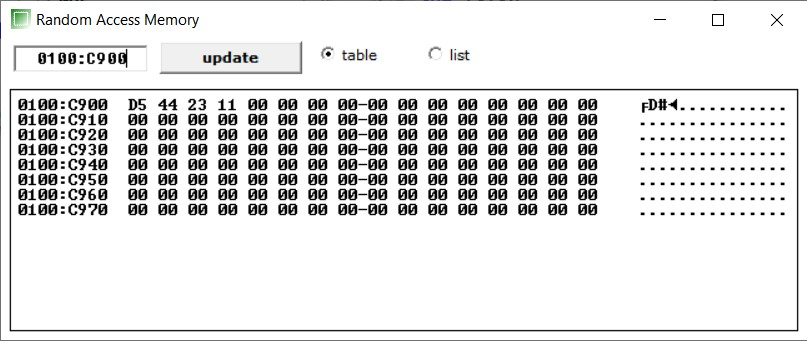
\includegraphics[width=1.0\textwidth]{EVEN_ODD_RAM} 
\caption{RAM Input for Q2}
\end{center}
\end{figure}

\subsubsection{Expectation}
BH: 01 \\
BL: 03 \\
That is 3 ODD and 1 EVEN number \\

%----------------------------------------------------------------------------------------
%	subsection 4
%----------------------------------------------------------------------------------------
\break
\subsubsection{Emulator}
\begin{figure}[h]
\begin{center}
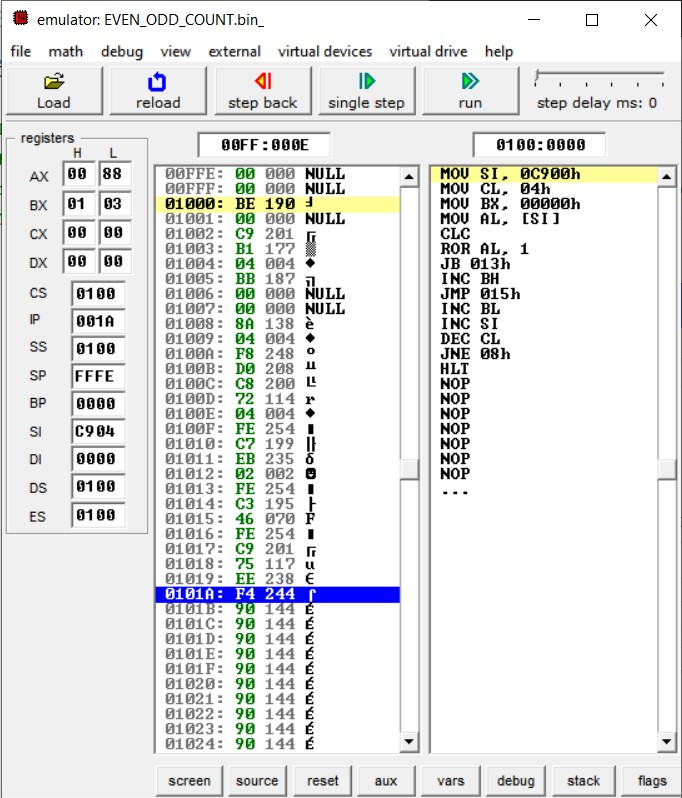
\includegraphics[width=0.8\textwidth]{EVEN_ODD_COUNT} 
\caption{STACK Output for Q2}
\end{center}
\end{figure}


%----------------------------------------------------------------------------------------
%	Question 3
%----------------------------------------------------------------------------------------

\break
\section{Question 3}
%----------------------------------------------------------------------------------------
%	subsection 2
%----------------------------------------------------------------------------------------

\subsection{Aim}
Write the assembly language program for 8086 MP to arrange the array of numbers stored in memory in ascending order.

%----------------------------------------------------------------------------------------
%	subsection 2
%----------------------------------------------------------------------------------------

\subsection{Program}
\subsubsection{Code}
\inputminted{nasm}{"C:/Users/aadit/Documents/BTech/5th Semester/MC Lab/8086 Pgrm 1/SORT.asm"}

\subsubsection{Emulator}

\begin{center}
\begin{tabularx}{1.0\textwidth} { 
  | >{\centering\arraybackslash}X 
  | >{\centering\arraybackslash}X 
  | >{\centering\arraybackslash}X | }
 \hline
\textbf{Address  (CS:0100, IP:0000)} &\textbf{Machine code}&\textbf{Instruction} \\
  \hline
 01000 & BF, 04 & MOV CL, 04H \\ 
  \hline
   01002 & FE, C9 & DEC CL \\ 
  \hline
   01004 & BE, 00, C9 & MOV SI, 0C900H \\  
   \hline
   01007 & B5, 04 & MOV CH, 04H \\
   \hline
   01009 & FE, CD & DEC CH  \\
   \hline
   0100B & 8A, 04 & MOV AL, [SI]  \\
   \hline
   0100D & 46 & INC SI \\
   \hline
   0100E & 3A, 04 & CMP AL, [SI] \\
   \hline
   01010 & 72, 06 & JB 018H \\
    \hline
   01012 & 86, 04 & XCHG [SI], AL \\
    \hline
   01014 & 4E & DEC SI \\
    \hline
   01015 & 86, 04 & XCHG [SI], AL \\
   \hline
   01017 & 46 & INC SI \\
   \hline
   01018 & FE, CD & DEC CH \\
  \hline
  0101A & 75, EF & JNE 0BH \\
  \hline
0101C & FE, C9 & DEC CL \\
  \hline
  0101E & 75, E4 & JNE 04H \\
  \hline
  01020 & F4 & HLT \\  
  \hline
\end{tabularx}
\end{center}

%----------------------------------------------------------------------------------------
%	subsection 3
%----------------------------------------------------------------------------------------
\break
\subsection{Result}
\subsubsection{Input}
\begin{figure}[h]
\begin{center}
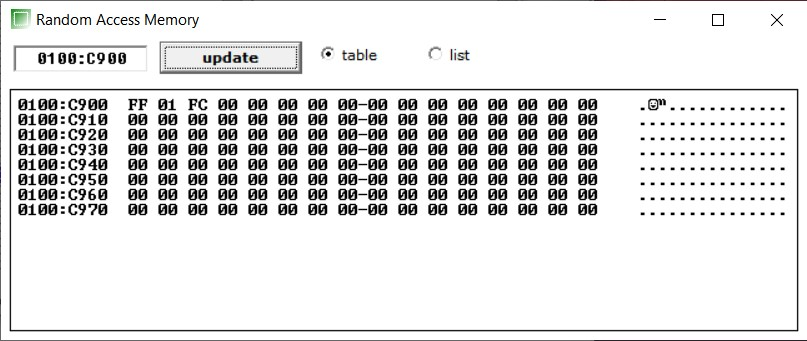
\includegraphics[width=1.0\textwidth]{SORT_IN} 
\caption{RAM Input for Q1}
\end{center}
\end{figure}

\subsubsection{Expectation}
0100:C900   00 01 FC FF \\

%----------------------------------------------------------------------------------------
%	subsection 4
%----------------------------------------------------------------------------------------
\break
\subsubsection{Emulator}
\begin{figure}[h]
\begin{center}
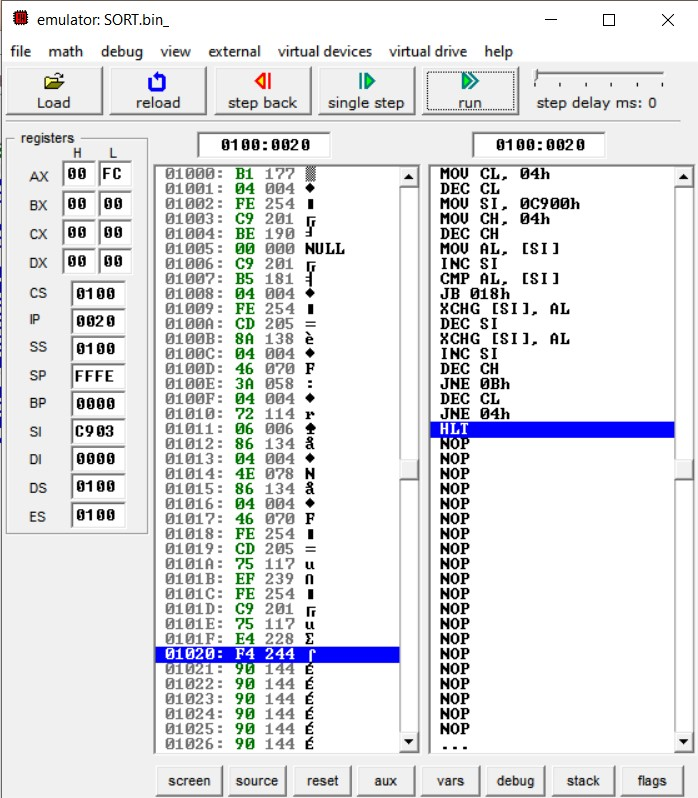
\includegraphics[width=0.6\textwidth]{SORT_OUT1} 
\caption{STACK Output for Q3}
\end{center}
\begin{center}
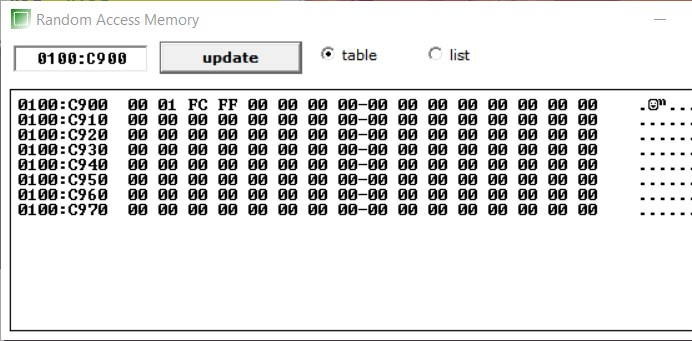
\includegraphics[width=0.65\textwidth]{SORT_OUT2} 
\caption{RAM Output for Q3}
\end{center}
\end{figure}
\end{document}